\chapter{Лекция}
\label{ch:intro}

На прошлом занятии мы рассматривали архитектуру простого передатчика и то, как в нем формируется и отправляется сигнал.

На этом занятии разберем архитектуру простого приемника и то, как он принимает сигнал и преобразует его обратно в данные.

\section*{\textbf{Архитектура простого приемника}}

\begin{figure}[H]
    \centering
    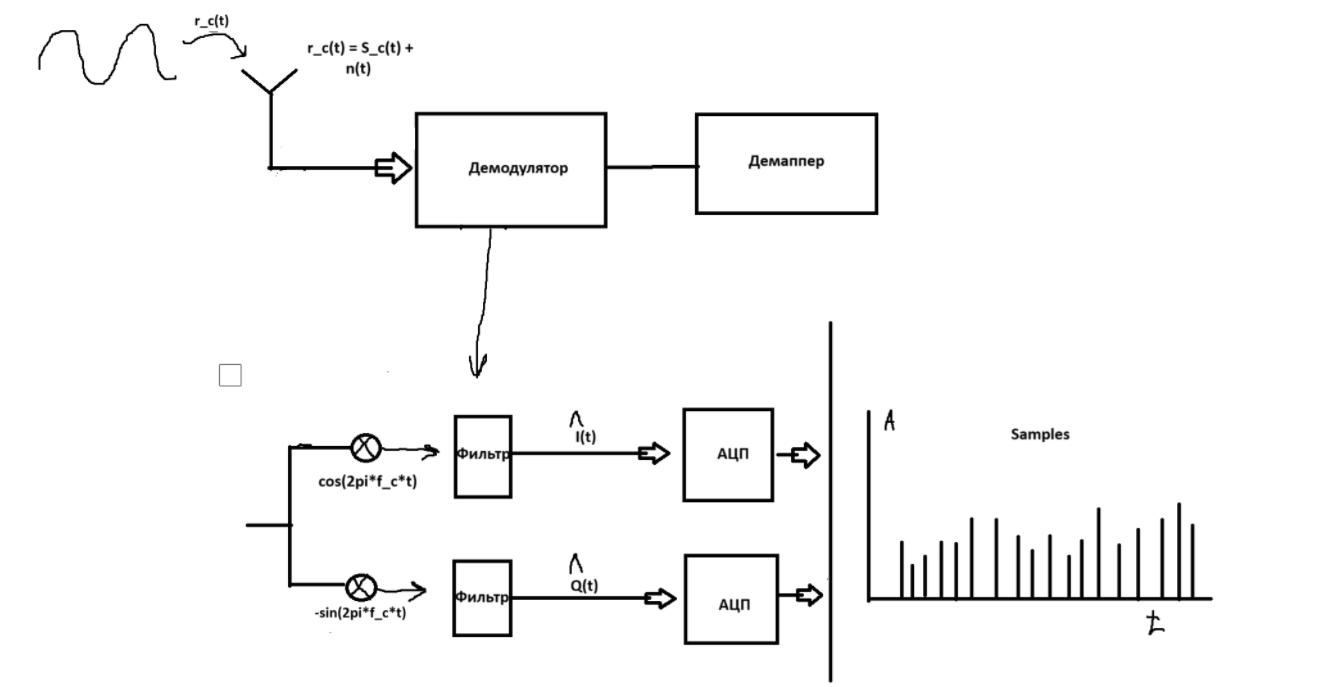
\includegraphics[width=0.8\textwidth]{rx_arch.png}
    \caption{Архитектура простого приемника}
\end{figure}

Сигнал поступает на антенну приемника и преобразуется в колебание электрического тока. Первым делом нам нужно выделить из этого
высокочастотного сигнала сигнал низкой частоты, т.к с низкочастотным сигналом работать проще и вся информаци содержится именно в нем.
Для этого подаем сигнал на демодулятор \\

\textbf{Демодуляция} - процесс, обратный модуляции колебаний, выделение информационного (модулирующего) сигнала из 
модулированного колебания высокой (несущей) частоты.  При передаче цифровых сигналов в результате демодуляции получается 
последовательность символов, передающих исходную информацию (I(t) и Q(t)).

\section*{\textbf{Принцип работы демодулятора}}

На схеме видим, что поступивший в демодулятор сигнал проходит через цепь, в которой он перемножается на несущие $cos(\omega_ct)$ и
$-sin(\omega_ct)$. Но как это помогает нам узнать низкочастотный сигнал? В логике этих перемножений лежит достаточно простая
математика: \\

Вспомним из прошлого занятия, какой сигнал по итогу мы отправляли в радиоканал:

\begin{figure}[H]
    \centering
    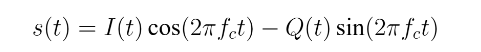
\includegraphics[width=0.8\textwidth]{rx_signal.png}
    \caption{Отправляемый сигнал}
\end{figure}

Вспомним математику 11 класса 

\begin{figure}[H]
    \centering
    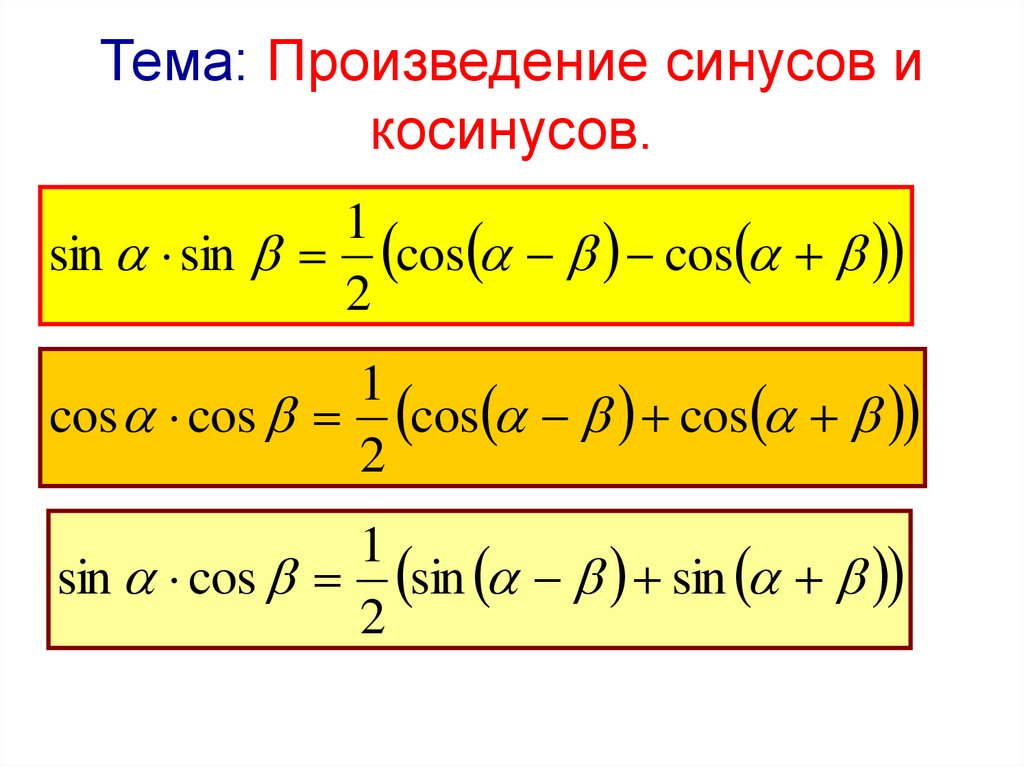
\includegraphics[width=0.8\textwidth]{triga.png}
    \caption{Тригонометрические формулы}
\end{figure}

Теперь произведем перемножения входного сигнала на несущие:


$$(I(t)cos(\omega_ct)-Q(t)(t)sin(\omega_ct)) * cos(\omega_ct)$$

$$= I(t)cos(\omega_ct)cos(\omega_ct) - Q(t)sin(\omega_ct)cos(\omega_ct)$$

$$= \frac{I(t)}{2}(cos(2\omega_ct) + cos(0)) - \frac{Q(t)}{2}(sin(2\omega_ct) + sin(0))$$

$$= \frac{I(t)}{2}cos(2\omega_ct) - \frac{Q(t)}{2}sin(2\omega_ct) + \boxed{\frac{I(t)}{2}}$$

У нас получилось выделить синфазную компоненту I(t). \\

Проделаем те же действия с умножением на sin

\[
(I(t)\cos(\omega_c t) - Q(t)\sin(\omega_c t)) \cdot \sin(\omega_c t)
\]

\[
= I(t)\cos(\omega_c t)\sin(\omega_c t) - Q(t)\sin^2(\omega_c t)
\]

\[
= \frac{I(t)}{2}\sin(2\omega_c t) - \frac{Q(t)}{2}(1 - \cos(2\omega_c t))
\]

\[
= \frac{I(t)}{2}\sin(2\omega_c t) + \frac{Q(t)}{2}\cos(2\omega_c t) - \boxed{\frac{Q(t)}{2}}
\]

Получили квадратурную компоненту Q(t). \\


Помимо самих компонент остались и другие сигналы, которые нам не нужны, поэтому с помощью фильтра уберем их. На выходе получим чистые
$\frac{I}{2}$ и $-\frac{Q}{2}$. Можно заметить, что после извлечения символов их амплитуда упала вдвое. Эта проблема решается
путем усиления (на схеме не отображено)\\

Далее компоненты поступают на АЦП, где будут "нарезаны" на семплы. В этих семплах нужно произвести символьную синхронизацию.

\endinput

